\documentclass[11pt,a4paper]{article}
\usepackage[margin=24mm]{geometry}
\usepackage[T1]{fontenc}
\usepackage{lmodern}
\usepackage{amsmath,amssymb}
\usepackage{booktabs,tabularx,array}
\usepackage{graphicx}
\usepackage{tikz}
\usetikzlibrary{arrows.meta,positioning,calc}
\usepackage{pgfplots}
\usepgfplotslibrary{groupplots}
\pgfplotsset{compat=1.18}
\usepackage[font=small,labelfont=bf]{caption}
\usepackage{placeins}
\usepackage{microtype}
\usepackage{titlesec}
\titlespacing*{\section}{0pt}{2.5ex plus 1ex}{1.3ex}
\titlespacing*{\subsection}{0pt}{2ex plus .5ex}{1ex}
\usepackage[numbers,sort&compress]{natbib}
\usepackage[hidelinks,breaklinks]{hyperref}
\usepackage{xurl}
\definecolor{steel}{HTML}{315D7B}
\definecolor{rust}{HTML}{AE5939}
\definecolor{cluster0}{HTML}{347CA8}
\definecolor{cluster1}{HTML}{BF6D20}
\definecolor{cluster2}{HTML}{378951}
\definecolor{cluster3}{HTML}{BE4545}
\definecolor{cluster4}{HTML}{855AA5}
\definecolor{cluster5}{HTML}{8B6657}
\definecolor{cluster6}{HTML}{B85D8B}
\definecolor{cluster7}{HTML}{64757B}
\definecolor{cluster8}{HTML}{A39037}
\definecolor{cluster9}{HTML}{168A94}
\tikzset{box/.style={draw=steel!70,fill=steel!5,rounded corners=1pt,align=center,text width=3.1cm,minimum height=1.2cm,font=\small,inner sep=6pt},widebox/.style={box,text width=12.4cm,minimum height=1cm},arrow/.style={-{Latex[length=2mm]},thick,draw=steel!80}}
\setlength{\parindent}{0pt}
\setlength{\parskip}{6pt}
\setlength{\emergencystretch}{2em}
\renewcommand{\topfraction}{.95}
\renewcommand{\bottomfraction}{.9}
\renewcommand{\textfraction}{.05}
\renewcommand{\floatpagefraction}{.75}
\newcommand{\diagram}[1]{\resizebox{\linewidth}{!}{\input{figures/#1.tex}}}

% Cluster map with aligned cluster numbers (make_figures.py) beside the
% original Python dendrogram from the study run (import_python_figures.py).
\newcommand{\clusterpair}[1]{%
\begin{minipage}[c]{.58\linewidth}
\centering\includegraphics[width=\linewidth]{figures/cluster_map_#1.pdf}
\end{minipage}\hfill%
\begin{minipage}[c]{.41\linewidth}
\centering\includegraphics[width=\linewidth]{figures/python/dendrogram_#1.png}
\end{minipage}}

\begin{document}
\section*{Three cross-sectional study diagram atlas}
Manuscript figures: editable TikZ and PGFPlots diagrams, together with the original Python-generated cluster maps and dendrograms. Cluster-map identifiers in the Python figures are local to each date.
\clearpage
\begin{figure}[p]
\centering
\diagram{population}
\caption{Index populations and continuity. The flow population has 39 complete histories; every date-specific fit retains all 41 instruments.}\end{figure}
\clearpage
\begin{figure}[p]
\centering
\diagram{windows}
\caption{Dependence across the three cross-sections. Bars depict trailing annual market windows schematically; fundamentals follow their recorded issuer reporting dates, not these uniform windows.}\end{figure}
\clearpage
\begin{figure}[p]
\centering
\diagram{pipeline}
\caption{Repeated cross-sectional study workflow. The preprocessing reference carries forward, while each date receives a fresh representation and partition.}\end{figure}
\clearpage
\begin{figure}[p]
\centering
\diagram{alignment}
\caption{Matching clusters with an observed overlap example. Five of the eight earlier group-1 members occupy the later group-1 match. This local example illustrates the similarity calculation; the actual assignment optimises all group pairs jointly.}\end{figure}
\clearpage
\begin{figure}[p]
\centering
\diagram{quality}
\caption{The same partitions evaluated in two geometries. UMAP has the stronger embedding silhouette at every date; this advantage does not consistently hold in the underlying financial features.}\end{figure}
\clearpage
\begin{figure}[p]
\centering
\diagram{seed_variability}
\caption{Ten pairwise adjusted Rand indices from five UMAP seeds at each date. Points are offset horizontally for readability; red segments mark the means. Pairs share fitted partitions and are dependent, so the spread is not a confidence interval or an empirical null for temporal switches.}\end{figure}
\clearpage
\begin{figure}[p]
\centering
\pythonclusterpair{2025-06-30}
\caption{Original Python cluster map and dendrogram for 2025-06-30. All 41 instruments are included. Cluster numbers in the map are local to this date; tree branch colours are independent of map colours.}
\end{figure}
\clearpage
\begin{figure}[p]
\centering
\pythonclusterpair{2025-12-31}
\caption{Original Python cluster map and dendrogram for 2025-12-31. All 41 instruments are included. Cluster numbers in the map are local to this date; tree branch colours are independent of map colours.}
\end{figure}
\clearpage
\begin{figure}[p]
\centering
\pythonclusterpair{2026-06-30}
\caption{Original Python cluster map and dendrogram for 2026-06-30. All 41 instruments are included. Cluster numbers in the map are local to this date; tree branch colours are independent of map colours.}
\end{figure}
\clearpage
\begin{figure}[p]
\centering
\diagram{flows}
\caption{Cluster membership across the three decision dates for the 39 continuously observed instruments. Bold tickers change aligned group at least once. APN, MNP, GLN and PAN are excluded only from this complete-history view. Colours and labels identify aligned groups, not sectors; vertical positions are layout.}\end{figure}
\clearpage
\begin{figure}[p]
\centering
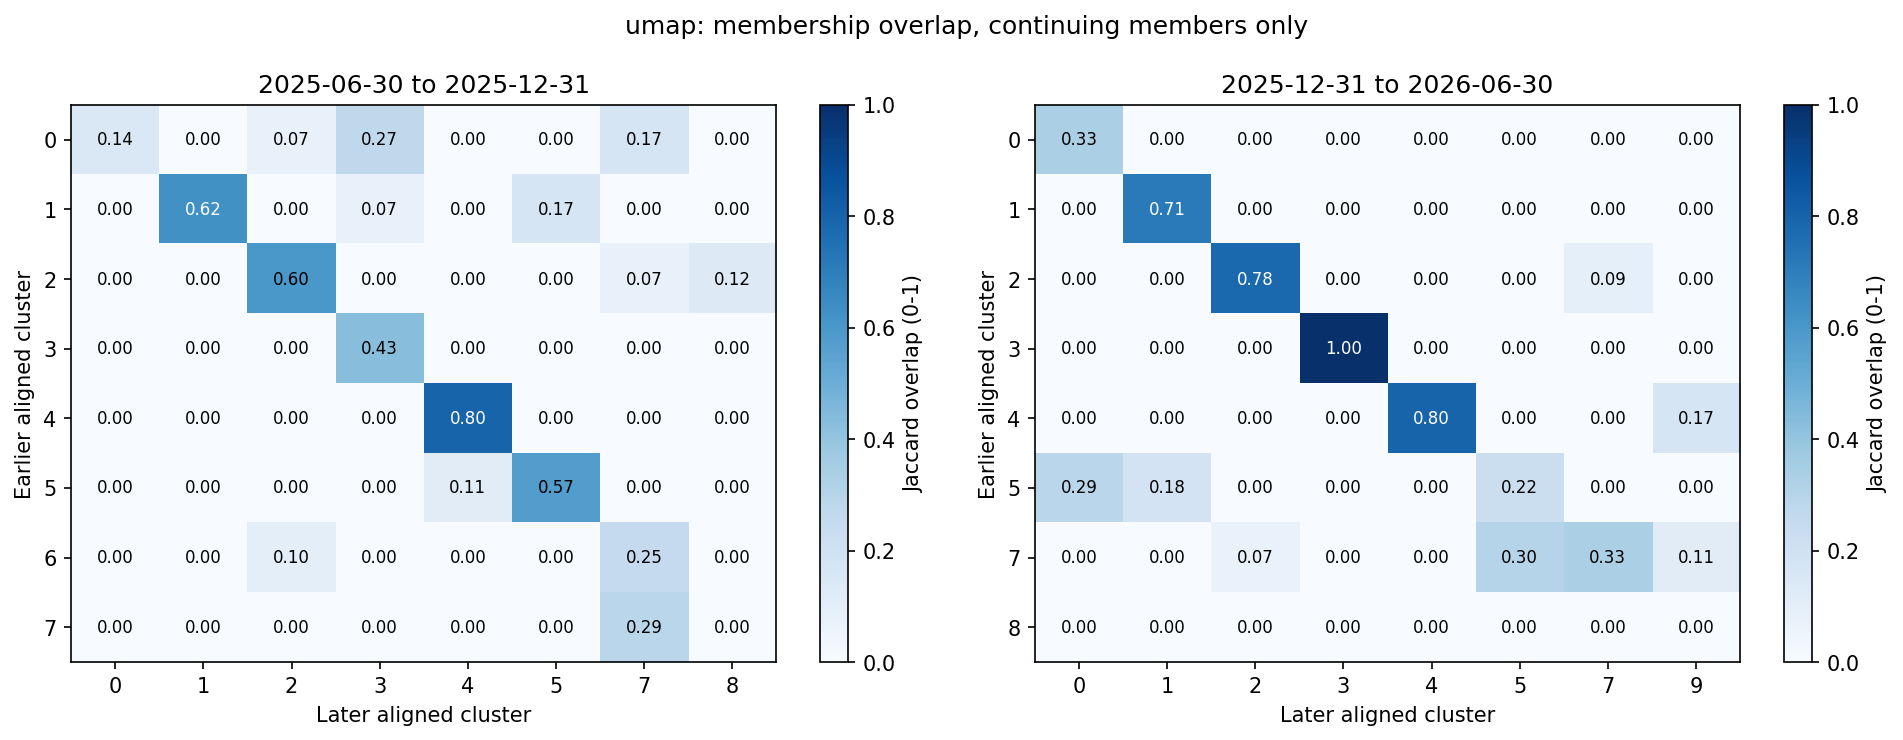
\includegraphics[width=\linewidth]{figures/python/jaccard.png}
\caption{Jaccard overlap among the 40 continuing members in each adjacent comparison. Each cell uses the common eligible universe for that period. Numeric values are given explicitly; a zero denotes no shared continuing member.}\end{figure}
\clearpage
\begin{figure}[p]
\centering
\diagram{profile0}
\caption{June 2025 aligned-cluster median deviations from the same-date median, in June 2025 MinMax units. Counts include all 41 date-specific instruments. Colours use the same range across the three figures; gaps in cluster numbers reflect retired identifiers.}\end{figure}
\clearpage
\begin{figure}[p]
\centering
\diagram{profile1}
\caption{December 2025 aligned-cluster median deviations from the same-date median, in June 2025 MinMax units. Counts include all 41 date-specific instruments. Colours use the same range across the three figures; gaps in cluster numbers reflect retired identifiers.}\end{figure}
\clearpage
\begin{figure}[p]
\centering
\diagram{profile2}
\caption{June 2026 aligned-cluster median deviations from the same-date median, in June 2025 MinMax units. Counts include all 41 date-specific instruments. Colours use the same range across the three figures; gaps in cluster numbers reflect retired identifiers.}\end{figure}
\clearpage
\begin{figure}[p]
\centering
\diagram{feature_sensitivity}
\caption{Complete-history outcomes under four feature representations using the UMAP recipe. Each bar contains the same 39 continuously observed instruments; four partial histories are outside every bar. The counts are representation-dependent and are not estimates of true economic change.}\end{figure}
\clearpage
\begin{figure}[p]
\centering
\diagram{cluster_count}
\caption{Cluster-count sensitivity from two to twelve groups. Blue lines show financial-feature scores and red lines embedding scores. Eight groups remain the reference specification.}\end{figure}
\clearpage
\begin{figure}[p]
\centering
\diagram{evidence}
\caption{Interpretation of the screening results. Peer-group changes, financial profiles and multivariate distance provide separate reasons for analyst follow-up. External validation is required before identifying a confirmed economic anomaly.}\end{figure}
\end{document}
